\chapter{Практическое применение модели}
Понимание того, как будет работать модель на практике, важная часть исследовательской деятельности. На основе экспериментов можно будет давать практические рекомендации по подбору параметров, спецификации при использовании. Правильная постановка эксперимента позволит сравнить предложенный метод с бейзлайном.

\section{Описание данных}
\note{Этап создания алгоритмов}
Инфраструктура, созданная в компании, предусматривает взаимодействие с широким кругом лиц, которые внештатно создают торговые стратегии, получая за это небольшое вознаграждение. При написании алгоритма можно:
\begin{enumerate}
	\item выбрать торгуемые активы
	\item задать периодичность, с которой работает алгоритм
	\item собирать любые статистики с предыдущих периодов
	\item произвольным образом реструктурировать портфель основываясь на прошлой информации
\end{enumerate}
Обладая навыками программирования на \texttt{Python}, можно написать любую стратегию, которая использует только рыночные данные. Алгоритмов огромное количество, более 700 000, большинство из этих алгоритмов написаны энтузиастами. В отличие от рыночных активов, которых ограниченное количество, алгоримов гораздо больше. Это открывает широкие возможности для применения портфельной теории для создания диверсифицированного портфеля.

\note{Этап селекции алгоритмов}
Тем не менее, применять портфельную теорию проблематично. Для такого количества временных рядов длина ряда слишком мала. Расчет даже ковариационной матрицы требует огромных вычислительных мощностей и памяти. Для решения этой проблемы существует этап предварительного отбора алгоритмов, этап селекции. В инфраструктуре разработана модель, которая выбирает наиболее стабильные из совокупности\footnote{Детали реализации защищены NDA}. После этого этапа остается около 150 торговых стратегий, которые и были использованы для тестирования модели динамики.

\section{Проверка предпосылок и выбор спецификации модели}
Перед непосредственно оценкой спецификаций модели динамики доходностей, был проведен эмпирический анализ алгоритмов, отобранных после селекции. Основной его задачей было выяснить, какие предпосылки себя оправдывают и какая спецификация наиболее полно описывает распределение доходностей во времени. 

\begin{figure}[h]
	\centering
	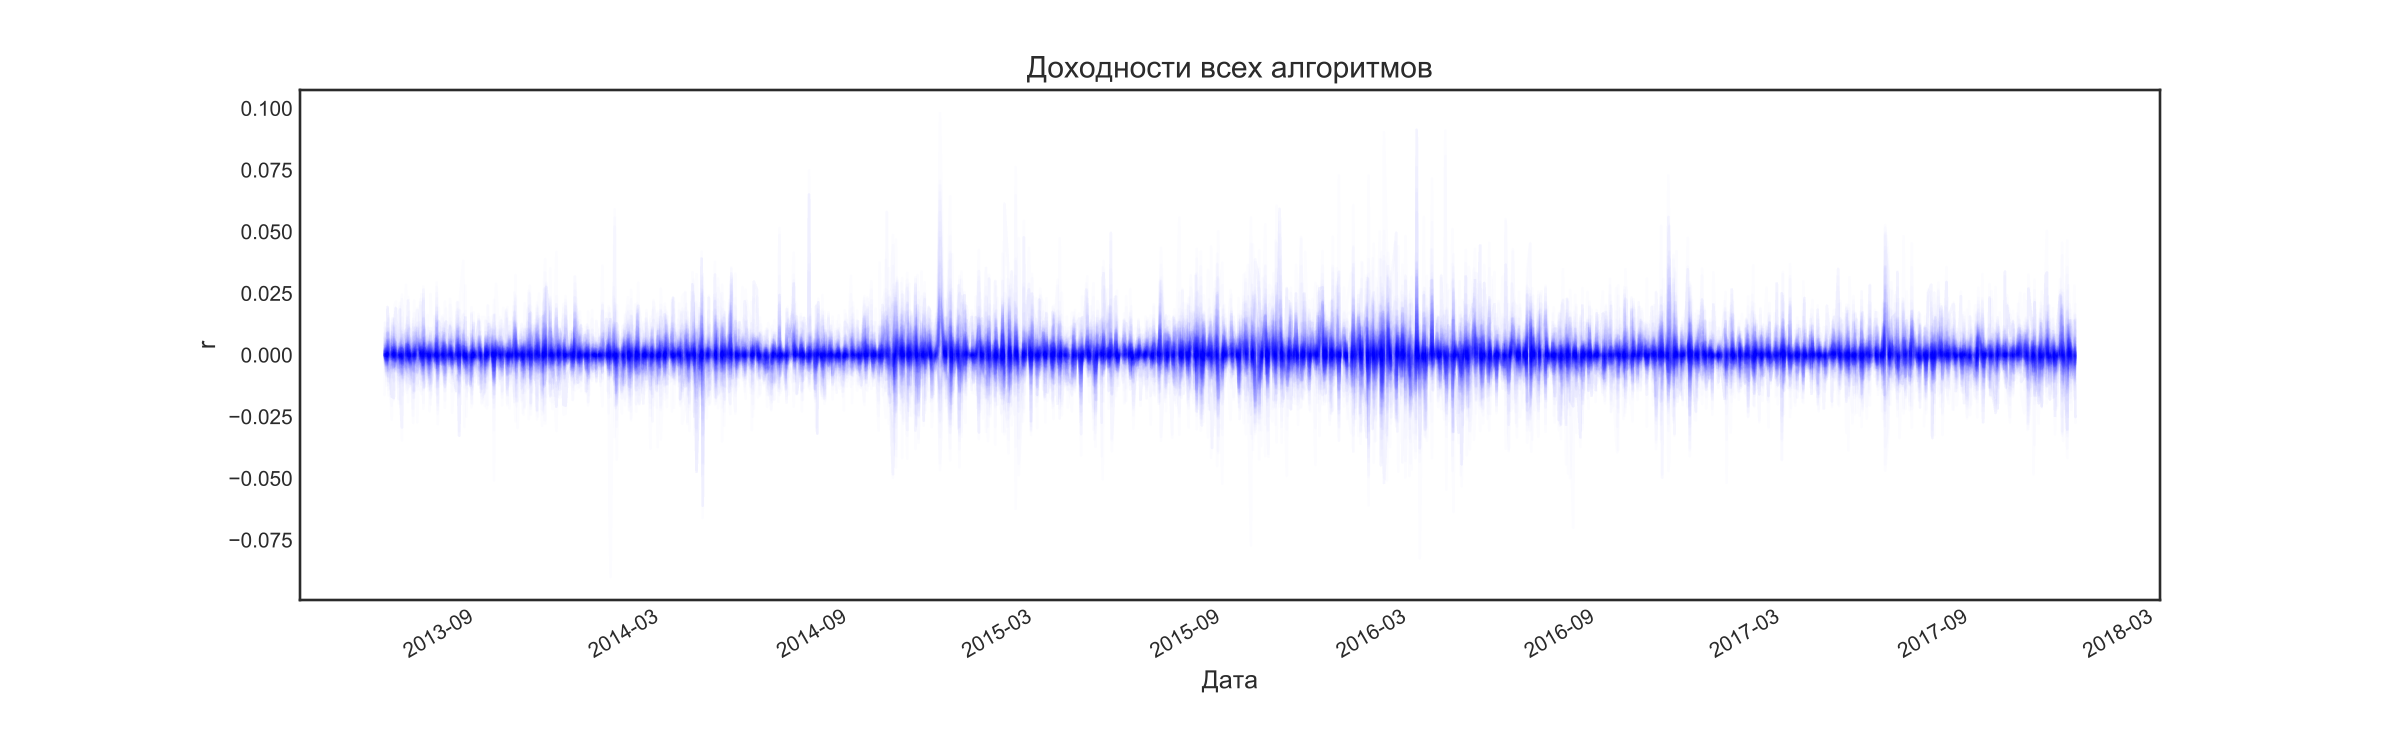
\includegraphics[width=\linewidth]{Thesis/images/returns-all}
	\caption{Доходности всех алгоритмов, на графике наблюдается непостоянная волатильность}
	\label{fig:allreturns}
\end{figure}

Гипотеза о непостоянстве волатильности находит свое подтверждение в графике распределения доходностей всех алгоритмов во времени (Рисунок \ref{fig:allreturns}). На нем видны периоды с высокой волатильностью. Более того, эффект наблюдается во многих алгоритмах в рамках одного периода.	

\begin{wrapfigure}{r}{.49\linewidth}
	\centering
	\includegraphics[width=\linewidth]{Thesis/images/returns-monthly}
	\caption{Распределение доходностей всех алгоритмов, сгруппированные по месяцам}
	\label{fig:monthlyreturns}
\end{wrapfigure}

Первичный анализ наличия сезонности в общем поведении алгоритмов не дал результатов: распределение доходностей, сгруппированных по месяцам выглядит однородно (Рисунок \ref{fig:monthlyreturns}).

\begin{figure}[h]
	\centering
	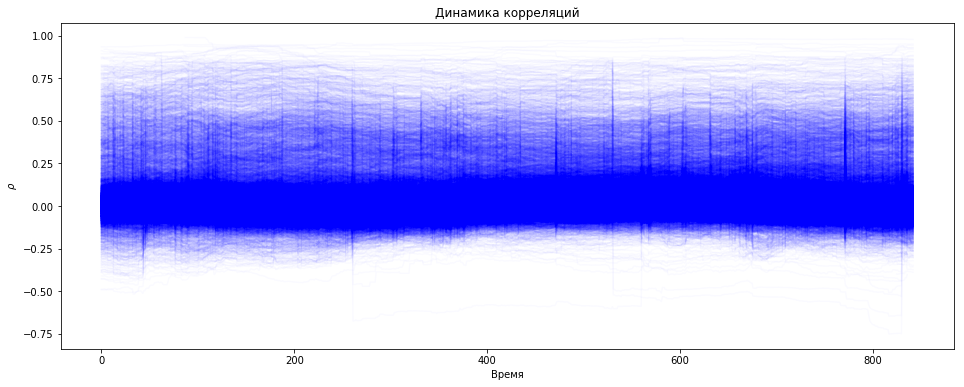
\includegraphics[width=\linewidth]{Thesis/images/correlations}
	\caption{График динамики корреляций между торговыми стратегиями. Попарные корреляции были посчитаны за период 2013-2017 с окном 300 дней. Не наблюдается существенного изменения корреляций за этот период.}
	\label{fig:correlations}
\end{figure}
Этап селекции имел важные последствия на спецификацию модели. Предположение о динамике корреляций оказалось не состоятельным (Рисунок \ref{fig:correlations})\footnote{Теста}. В данных не наблюдается существенного изменения корреляций для большой группы торговых стратегий. Значительное количество траекторий значительно отдалены от нуля. Тем не менее, на основе этого графика сделать вывод о структуре ковариационной матрицы (блочная/плотная) нельзя. В сложившейся ситуации этот анализ избыточен, так как семейство моделей с плотной матрицей ковариации включает в себя подмножество тех, что имеют блочную структуру. 

Выводы, которые можно сделать на основе проведенного анализа:
\begin{itemize}
	\item присутствует стохастическая волатильность
	\item сезонность в данных отсутствует или незначительна
	\item корреляции относительно стабильны во времени
	\item большинство корреляций околонулевые
\end{itemize}

Основываясь на них, остается сфокусироваться на двух спецификациях, которые не учитывают динамику корреляций:
\begin{itemize}
	\item модель без корреляций \eqref{eq:nocorr}
	\item модель со статичными корреляциями \eqref{eq:staticcorr}
\end{itemize}

Корреляционная матрица стабильна во времени, существуют негативные корреляции, много корреляций отличных от нуля, она имеет плотную структуру, которую невозможно учесть, используя блочной структуры матрицу. Модель, учитывающая динамику корреляций, не подходит для моделирования стохастического процесса доходностей торговых стратегий. Более того, в экспериментах модель страдала от ряда проблем:
\begin{itemize}
	\item Долгая фаза адаптации ковариационной матрицы <<пропозал>>\footnote{В английской литературе оно называется proposal distribution} распределения
	\item Долгая сходимость марковской цепи (более 10000 итераций)
	\item Продолжительные расчеты для оценки модели (около 12 ч.)
	\item Модель не работала для моделирования динамики большой группы алгоритмов
\end{itemize}

\section{Реализация моделей и сравнительный анализ в рамках портфельной оптимизации}
\note{Описание поставленного эксперимента}
Для качественных выводов о работе предложенного метода составления портфеля недостаточно оценить одну модель на подвыборке алгоритмов, так как это может быть случайный успех или неудача. Для проведения эксперимента на реальных данных, был использован метод бутстрап \citep{grimshaw1995} и разделение выборки на обучающую и тестовую.

\textbf{Постановка эксперимента:}
\begin{itemize}
	\item Всего 4 года наблюдений
	\item Обучающая выборка -- первые два года
	\item Тестовая выборка -- последние два года
	\item Сгенерировано 400 выборок алгоритмов размера 20 из 150 без повторений
	\item Тремя методами: предложенными \eqref{eq:staticcorr}, \eqref{eq:nocorr} и по Марковицу, строятся портфели основываясь на данных обучающей выборки
	\item Считается критерий качества (коэффициент Шарпа) на тестовой выборке
\end{itemize}

\note{Параметры NUTS}
Для оценки апостериорных распределений параметров модели использовался алгоритм NUTS \citep{hoffman2011nuts}, при этом генерировалась выборка размера 3000 из этого распределения. Для оценки потребовались большие вычислительные мощности. Так, расчет модели на динамику 20-ти алгоритмов со статическими корреляциями \eqref{eq:staticcorr} занимает около 3х часов на 32х-ядерном сервере. Оценка модели без корреляций \eqref{eq:nocorr} занимает менее получаса. Весь эксперимент длился более месяца.

\note{Описание и трактовка результатов}
Результаты эксперимента предствлены на на рисунке \ref{fig:performance}. На первой строчке изображены распределения коэффициентов Шарпа, получаемые разными методами: методом Марковица (Mark, всегда черным цветом), через модель со статическими корреляциями (Corr) и без корреляций (Diag) соответственно. На второй строчке изображены распределения разности коэффициентов Шарпа полученных с помощью модели Corr и Diag, Corr и Mark, Diag и Mark. На третьей строчке изображена разность волатильности портфеля для Corr и Diag и далее плотности волатильности моделей Corr, Diag и Mark. Цветовая шкала означает значение параметра $\rho$ в функции полезности \eqref{eq:isoelastic}. Распределение коэффициента Шарпа на тестовом периоде находится значительно правее, что означает преимущество предложенного метода над ранее используемым аналогом. 

Из экспериментов следует, что предложенный алгоритм более устойчив при обучении, обладает необходимой обобщающей способностью для улучшения качества портфеля по ряду показателей. В целом не важно, какую спецификацию модели выбирать: дополнительное моделирование корреляций не принесло большой пользы, разница волатильности и коэффициентов Шарпа между моделью \eqref{eq:staticcorr} и \eqref{eq:nocorr} имеет сконцентрированное в нуле распределение.
\begin{figure}[h]
	\centering
	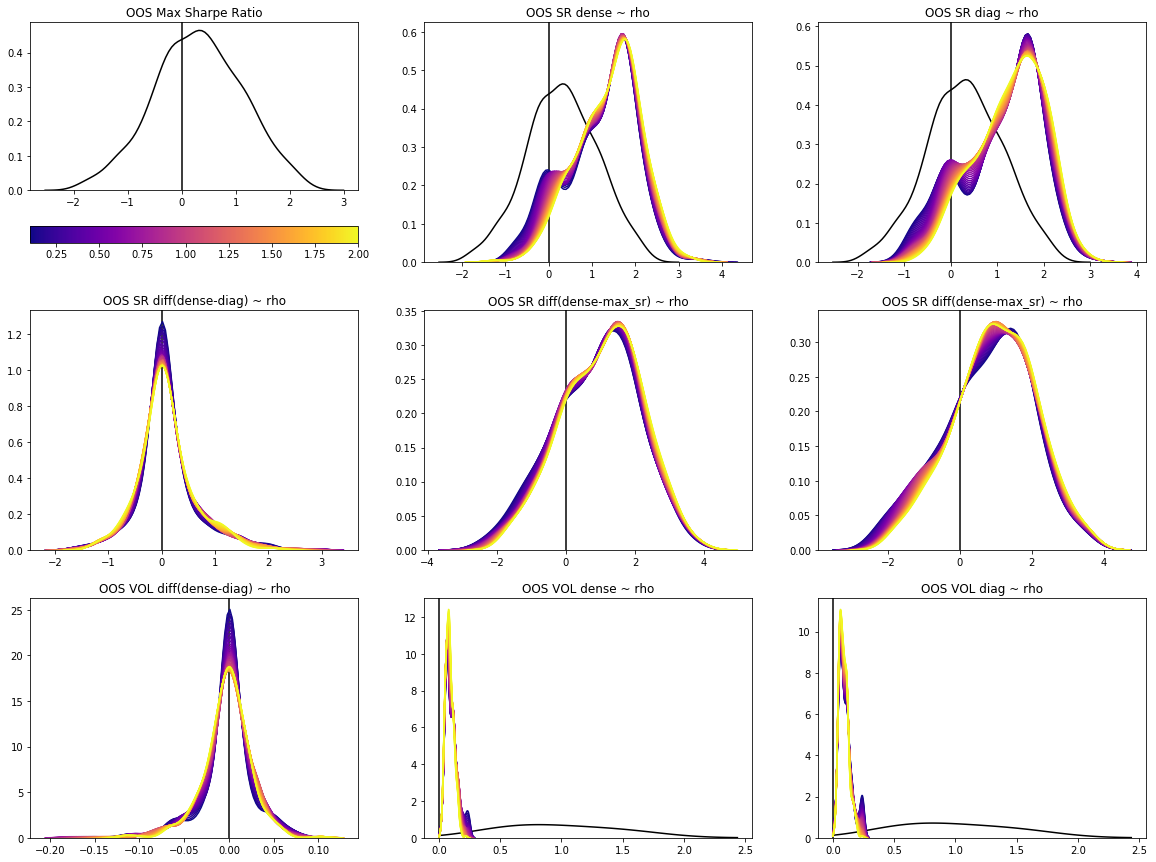
\includegraphics[width=\linewidth]{Thesis/images/performance}
	\caption{Сравнение коэффициента Шарпа на тестовой выборке байесовского (выделен цветом) и оптимального портфеля Марковица (черным) полученного методом бутстрап. Распределение коэффициента Шарпа на тестовом периоде находится значительно правее, что означает преимущество предложенного метода над ранее используемым аналогом. }
	\label{fig:performance}
\end{figure}
\\\\
\textbf{Основные выводы}
\begin{itemize}
	\item Коэффициент Шарпа: в 70\% случайно выбранных портфелях коэффициент Шарпа больше полученного методом Марковица
	\item Дисперсия получаемого портфеля новым способом ниже
	\item Моделирование корреляций не дает существенного преимущества перед моделью без них
\end{itemize}

